%===================================== CHAP 1 =================================

\chapter{Introduction}

In recent years there has been made substantial progress in the field of autonomous vehicles, and companies such as Google, Tesla and Uber are investing heavily in the development of autonomous cars. In Norway, with our maritime expertise and long coastline, a research field of interest has been autonomous ferries. Currently, Kongsberg Gruppen is developing the world's first zero emission, autonomous container feeder for Yara, which could be able to reduce diesel-powered truck journeys by around 40,000 trips per year \citep{yara}. In Trondheim, the development of an autonomous passenger ferry is ongoing \citep{autonom_trd}. 

\vspace{3mm}

\noindent
A crucial part of an autonomous system is the ability to sense and understand its surroundings. Sensors such as lidars and radars are good at measuring distance, and are used both in autonomous cars and ferries. This report investigates how cameras can be used to help an autonomous ferry generate information about its surroundings. The same problem has already been studied to some extent at the Rolls Royce Singapore Lab \citep{Prasad2016a} and  \citep{Prasad2016}, but it is still necessary to investigate this topic further. This report separates from their research by focusing on detection algorithms based on deep learning. 

\vspace{3mm}

\noindent
In the last years, image classification and object detection have developed rapidly. In 2012 there was a breakthrough in image classification when AlexNet won the ImageNet Large-Scale Visual Recognition Challenge by a large margin, using a Convolutional Neural Network (CNN) for the first time in the competition \citep{Krizhevsky2012}. This was achievable because of easier access to the required computational power and the increased amount of data needed for training of such networks. In the following years, several CNNs for image classification were developed, e.g. VGGnet (2014), GoogLeNet (2015) and Microsoft ResNet (2015). Today the best classification algorithms have surpassed human-level performance on the ImageNet dataset \citep{He}. This technology can be used for many interesting purposes, e.g. image colorization \citep{Zhang2016}, image captioning \citep{Karpathy2016} and to create the worlds best GO player \citep{Silver2016}.

\vspace{3mm}

\noindent
The advances in image classification have also led to new deep learning based object detection algorithms. Where image classification seeks to classify objects in an \textit{image}, object detection aims to localize different objects in an image, \textit{and classify them}. An example of the output of an object detection algorithm is given in figure \ref{fig:imdet}. 

\begin{figure}[h!]
\centering
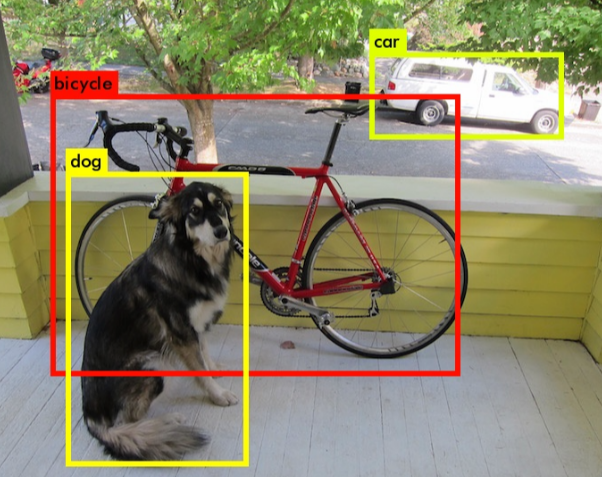
\includegraphics[scale=0.3]{images/imdet.png}
\caption{Output of an image detection algorithm, image from \citep{YOLOv1}.}
\label{fig:imdet}
\end{figure}


\noindent
This project aims to find a starting point for figuring out how well detection of maritime vessels can be, and to develop a user-friendly system that can be used to test and find statistics for detection algorithms trained on different data. Such a system simplifies identification of challenges in deep learning-based methods, and the work on trying to overcome these challenges can be simplified by having a consistent framework that automates this process. The scope of this thesis involves setting up a framework for testing and training of SSD and Yolo, to build a dataset, and to start the process of finding out what makes an object detector better at identifying maritime vessels in video.


\cleardoublepage